\section{Experimental Evaluation}
\label{Evaluation}
In this section, we report on our empirical evaluation of \crossrec on a cluster computing framework namely Spark with real world traces from Amazon~\cite{mcauley2013hidden} to analyze its prediction accuracy, privacy and scalability. We choose Spark as our cluster computing framework since the underlying framework to support \crossrec must be scalable and fault-tolerant.


\subsection{Experimental Setup}

\noindent{\bf Experimental platform.}
We perform all the experiments on a cluster consisting of 20 machines. Each machine is an Intel Xeon CPU E5520 @2.26GHz with 32 GB memory and 600 GB disk storage. The machines are connected through a 2xGigabit Ethernet (Broadcom NetXtremeII BCM5716).

\noindent{\bf Datasets.}
We use two sets of real traces from Amazon datasets~\cite{mcauley2013hidden}: \emph{movies} and \emph{books}. We use the ratings for the period from 2011 till 2013. The movies dataset consists of 743,735 ratings from 777,729 users for 168,105 movies where each user rated at least 10 movies. The books dataset consists of 1,424,135 ratings from 1,232,135 users for 567,731 books where each user rated at least 10 books. The ratings vary from 1 to 5 with an increment of 1 between the possible ratings. The overlapping users in these two datasets are those Amazon users who are present in both and are ascertained using their Amazon user-ids.
%From this original traces, we create two additional traces for our experiments. These dataset consists of users who rated at least 5 items in one domain. For users who rated in both the domains, these users also rated at least 10 items (5 from each domain). 

\noindent{\bf Evaluation metrics.}
We evaluate \crossrec along three complementary metrics: the recommendation \emph{quality} as perceived by the users in terms of prediction \emph{accuracy}, the degree of \emph{privacy} provided to the end-users in terms of the privacy parameters ($\epsilon, \epsilon'$) and the \emph{scalability} in terms of \emph{speedup} achieved in \crossrec by increasing the number of machines in the cluster.

{\it Accuracy.} We evaluate the accuracy of the predictions in terms of Mean Absolute Error (MAE). MAE computes the average absolute deviation between a predicted rating and the user's true rating. MAE is a standard metric used to evaluate state-of-the-art recommenders~\cite{breese1998empirical, herlocker1999algorithmic, shardanand1995social}. We assume that the predicted rating for an item $i$ is denoted by $p_i$ and the actual rating is denoted by $r_i$ in the test dataset. Then, the MAE for a test dataset, with $\mathcal{N}$ ratings, is computed as: $\frac{\sum _{i=1}^{\mathcal{N}}|p_i -r_i|}{\mathcal{N}}$. Given that $r_{min}$ and $r_{max}$ denotes the minimum and maximum ratings respectively, the following inequality always holds: $0< MAE < (r_{max}-r_{min})$. The lower the MAE, the more accurate the predictions.

%$$
%MAE=  \frac{\sum _{i=1}^{\mathcal{N}}|p_i -r_i|}{\mathcal{N}}
%$$  
%The lower the MAE, the more accurate the predictions.

{\it Privacy.} 
Our differential privacy guarantees are parameterized by the privacy parameters: $\epsilon$ for the Private Replacement Selection technique used for AlterEgo generation and $\epsilon'$ for the PNCF used for the private recommendation generation in \crossrec. According to the privacy literature~\cite{dwork2011firm, zhu2013differential,zhu2014effective}, $\epsilon=1$ or less would be suitable for privacy preserving purposes.

{\it Speedup.} We evaluate the speedup in terms of the time required for sequential execution ($T_1$) and the time required for parallel execution with $p$ processors ($T_p$). Amdahl's law~\cite{krishnaprasad2001uses} models the performance of speedup ($S_p$) as follows.
$$
S_p= \frac{T_1}{T_p}
$$
Due to the considerable size of the Amazon dataset, we compare the speedup on $p$ processors with respect to a minimum of $5$ processors ($T_5$) instead of a sequential execution ($T_1$).

\noindent{\bf Competitors.}
%The two systems (the two papers) which are used to compare with our system \crossrec along with the baseline approaches
We now present the recommenders against which we compare \crossrec. Existing recommendation schemes over several domains can be classified as follows.

{\it Linked-domain personalization.} The goal here is to recommend items in the target domain ($\mathcal{D}^T$) by exploring rating preferences aggregated from both source and target domains, i.e, to recommend items in $\mathcal{I}^T$ to users in $\mathcal{U}^S$ based on the preferences of users in $\mathcal{U}^S\; \cup \;\mathcal{U}^T$ for items in $\mathcal{I}^S \;\cup \;\mathcal{I}^T$. In this approach, ratings from multiple domains are aggregated into a single domain. Then, a traditional CF mechanism is applied over this aggregated single domain~\cite{sarwar2001item, cremonesi2011cross}. \textsc{Item-based-kNN} is a linked-domain personalization approach~\cite{sarwar2001item, cremonesi2011cross} where we use item-based collaborative filtering over the aggregated ratings over both the domains.

{\it Heterogeneous personalization.} The goal here is to recommend items in $\mathcal{I}^T$ to users in $\mathcal{U}^S$ based on the preferences of $\mathcal{U}^S$ for $\mathcal{I}^S$, $\mathcal{U}^T$ for $\mathcal{I}^T$ and $\mathcal{U}^S\; \cap\; \mathcal{U}^T$ for $\mathcal{I}^S\; \cup\; \mathcal{I}^T$. In this approach, the user similarities are first computed in both source and target domains. These domain-related similarities are then aggregated into the overall heterogeneous similarities. Finally, the $k$-nearest neighbors, used for recommendation computations, are selected based on these heterogeneous similarities~\cite{berkovsky2007cross}. In the \textsc{RemoteUser} approach~\cite{berkovsky2007cross}, the user similarities in source domain are used to compute the $k$ nearest neighbors for users who have not rated in target domain. Then user-based collaborative filtering is performed.

{\it Baseline prediction.} For sparse dataset, the baseline is provided by item-based average ratings~\cite{baltrunas2009context} or user-based average ratings~\cite{lemire2005slope}. The goal here is to predict based on the average ratings provided by users in $\mathcal{U}^S\; \cup\; \mathcal{U}^T$ for items in $\mathcal{I}^S\; \cup\; \mathcal{I}^T$. One of the most basic prediction scheme is the \textsc{ItemAverage} scheme where we predict that each item will be rated as the average over all users who rated that item~\cite{baltrunas2009context}. Note that though this technique gives a very good prediction of the actual rating but its not personalized.% and hence not suited for recommendation purpose.

We compare \crossrec with these three other systems namely: \textsc{Item-based-kNN}, \textsc{RemoteUser} and \textsc{ItemAverage}.

\noindent{\bf Evaluation scheme.} We partition the set of common users who rated both movies and books into \emph{training} and \emph{test} sets. For the test users, we hide their profile in the target domain (say books) and use their profile in the source domain (movies) to predict books for them. This strategy evaluates the accuracy of the predictions if the user did not rate any item in the target domain. Hence, we can evaluate the performance of \crossrec in the scenario where the test users did not rate any item in the target domain (cold-start). Additionally, if we hide part of the user profile in the target domain, then we can evaluate how \crossrec handles the scenario where the test users rated very few items in the target domain (sparsity). Furthermore, we denote the item-based variant of \crossrec as \crossrecib and the user-based variant as \crossrecub. Similarity for \npcrossrec, we denote the item-based variant of \npcrossrec as \npcrossrecib and the user-based variant as \npcrossrecub.
\subsection{Temporal Relevance}
In this section, we observe the temporal relevance effect for \crossrec, leveraging the item-based recommender, and then tune the temporal relevance parameter $\alpha$ accordingly. Figure~\ref{fig:temporal} demonstrates this effect compared to the approach without any temporal relevance effect ($\alpha=0$). We vary $\alpha$ between 0.01 to 0.3. Note that an item-based CF approach computes the predictions leveraging the target user's very few observed ratings on the nearest neighbors and given the very limited size of this set of ratings, any further amplification of $\alpha$ impacts predictions negatively as it reduces the contribution of old ratings furthermore. Hence, we set $\alpha$ for our experiments, based on Figure~\ref{fig:temporal}, to achieve optimal recommendation quality.% which guarantees better quality in all the four scenarios.
\begin{figure}
\begin{center}
\hspace{-3mm}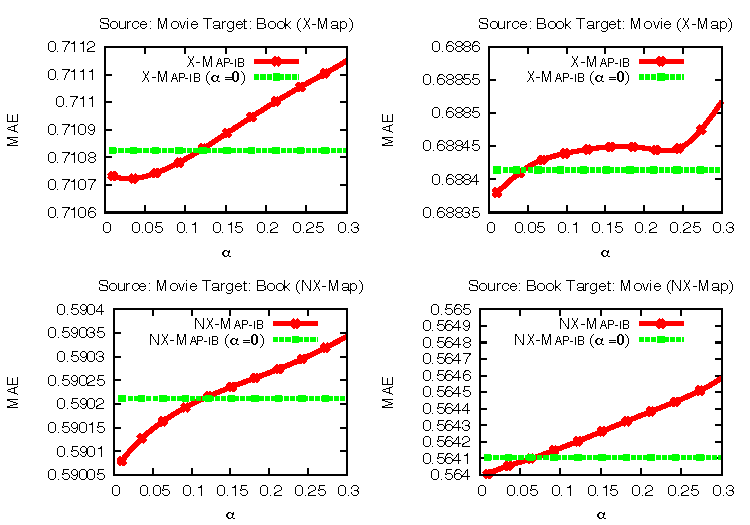
\includegraphics[height=2.4in,width=3.45in]{figures/Temporal_relevance.pdf}
\vspace{-8mm}
\caption{{\bf Temporal relevance (\crossrec, \npcrossrec).}}
\label{fig:temporal}
\end{center}
\end{figure}
\subsection{Privacy}
In this section, we tune the privacy parameters ($\epsilon, \epsilon'$) for \crossrec. Figures~\ref{fig:privacy_ib} and~\ref{fig:privacy_ub} demonstrate the effect of tuning the privacy parameters on the prediction quality in terms of MAE. We observe that the recommendation quality improves (lower MAE) as we decrease the degree of privacy (higher $\epsilon$, $\epsilon'$). For the following experiments, we select the privacy parameters as follows. For \crossrecub, we select $\epsilon=0.6$ and $\epsilon'=0.3$. For \crossrecib, we select $\epsilon=0.3$ and $\epsilon'=0.8$.\footnote{These parameters are selected from a range of possible values providing quality close to the optimal one as observed from Figures~\ref{fig:privacy_ib} and~\ref{fig:privacy_ub}.}

\begin{figure}[ht]
\vspace{-4mm}
\subfigure[\label{fig:privacy_ib_mb}]{\raisebox{0mm}{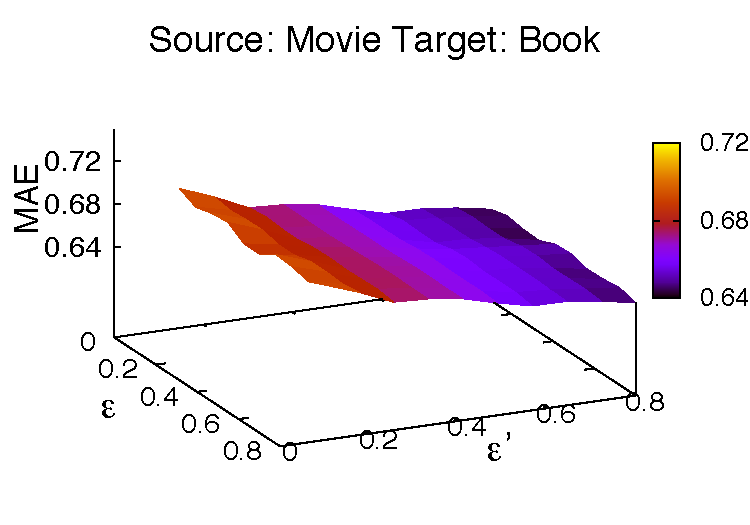
\includegraphics[width=0.23\textwidth,height=0.15\textheight]{figures/Privacy_ib_mb.pdf}}}
\subfigure[\label{fig:privacy_ib_bm}]{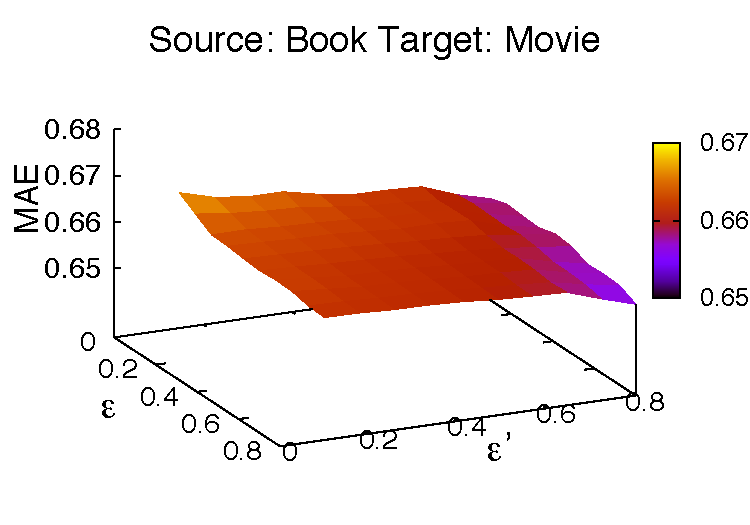
\includegraphics[width=0.24\textwidth,height=0.15\textheight]{figures/Privacy_ib_bm.pdf}}
\vspace{-6mm}
\caption{\bf Privacy trade-off (\crossrecib).}
\vspace{-1mm}
\label{fig:privacy_ib}
\end{figure}


\begin{figure}[ht]
\vspace{-2mm}
\subfigure[\label{fig:privacy_ub_mb}]{\raisebox{0mm}{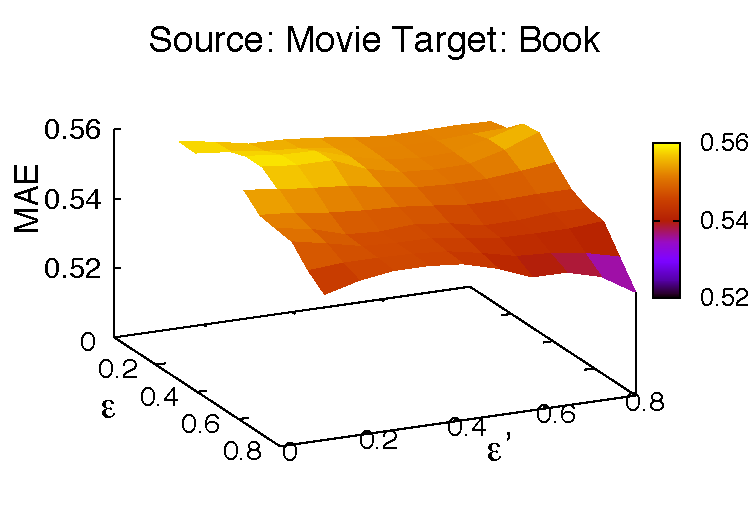
\includegraphics[width=0.23\textwidth,height=0.15\textheight]{figures/Privacy_ub_mb.pdf}}}
\subfigure[\label{fig:privacy_ub_bm}]{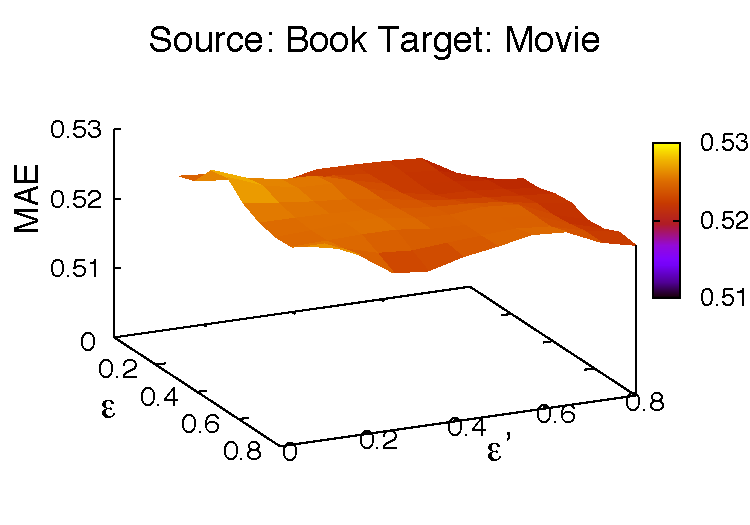
\includegraphics[width=0.24\textwidth,height=0.15\textheight]{figures/Privacy_ub_bm.pdf}}
\vspace{-6mm}
\caption{\bf Privacy trade-off (\crossrecub).}
\label{fig:privacy_ub}
\end{figure}


\subsection{Accuracy}
\label{eval:accuracy}
We now compare the accuracy of the predictions of \crossrec and \npcrossrec with the competitors.

\noindent{\bf Impact of top-k neighbors.}
First, we evaluate the quality in terms of MAE when the size of $k$ (neighbors in Equation~\ref{pred_ib_cf_time}) is varied. Figure~\ref{fig:Book2Movievaryk} demonstrates that \crossrecub and \npcrossrecub outperform the competitors by a significant margin of 30\% where the source domain is book and the target domain is movie. Also, Figure~\ref{fig:Movie2Bookvaryk} shows that \crossrecub and \crossrecib perform slightly better than the non-private competitors whereas \npcrossrec again outperforms the competitors by a margin of 18\% where the source domain is movie and the target domain is book. For all further experiments we consider $k$ as 50.

\begin{figure}[ht]
\vspace{-3mm}
\subfigure[\it \small Source:Book, Target:Movie \label{fig:Book2Movievaryk}]{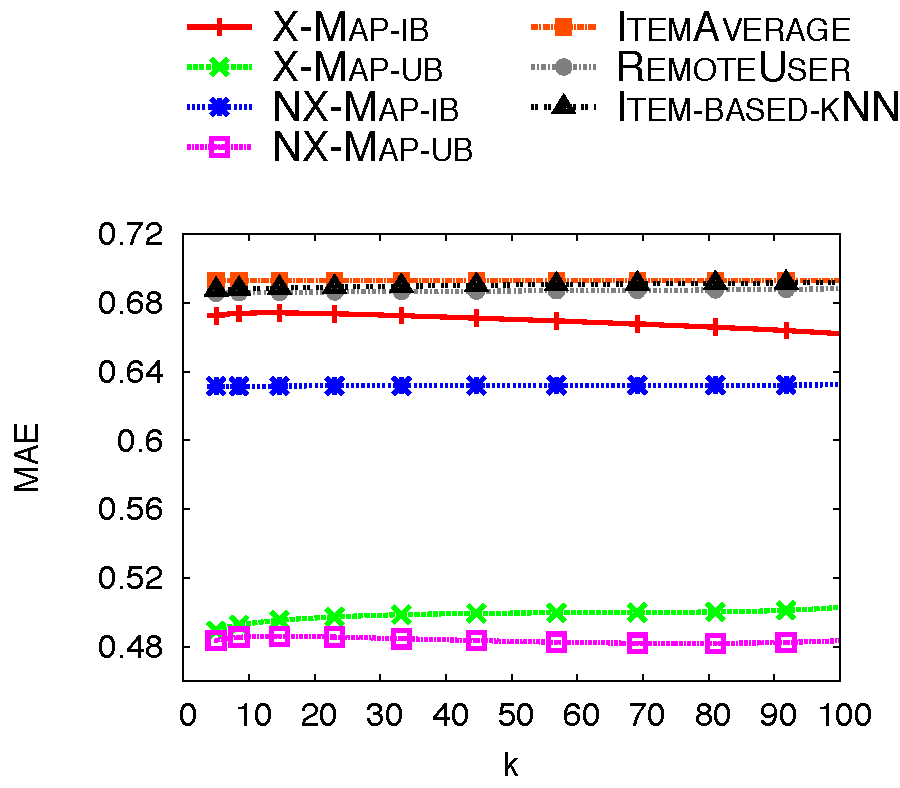
\includegraphics[width=0.245\textwidth,height=0.18\textheight]{figures/MAE_K_original.pdf}}\hspace{-1em}
\subfigure[\it \small Source:Movie, Target:Book \label{fig:Movie2Bookvaryk}]{\raisebox{1.4mm}{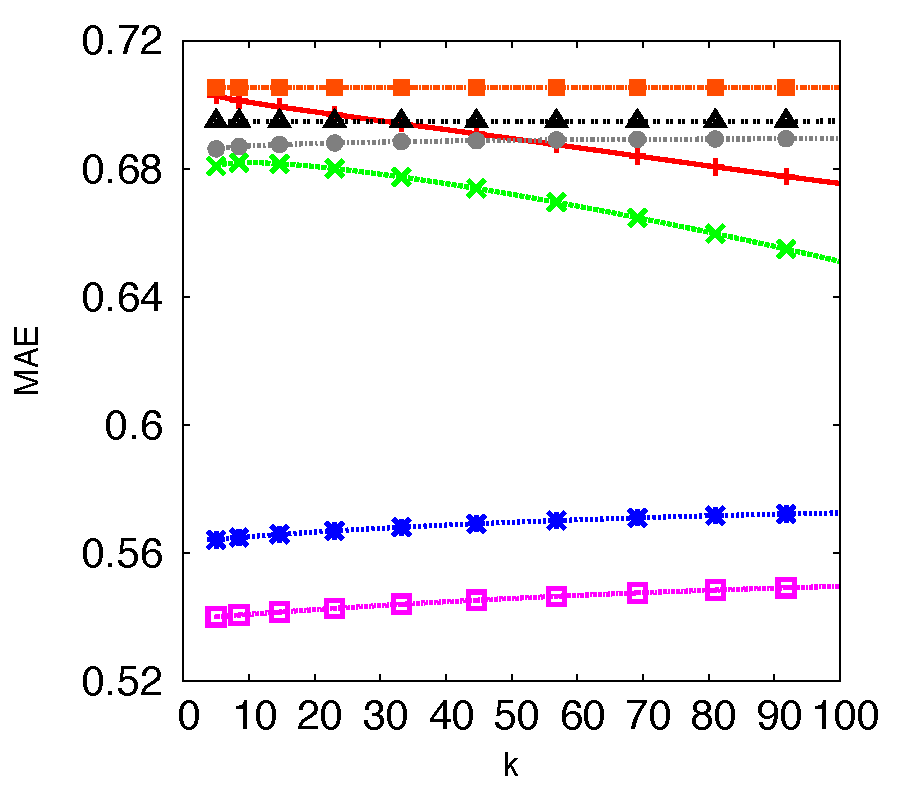
\includegraphics[width=0.245\textwidth,height=0.125\textheight]{figures/MAE_K_swapped.pdf}}}
\vspace{-6mm}
\caption{\bf MAE comparison with varying \emph{k}.}
\vspace{1mm}
\label{fig:varyK}
\end{figure}

\noindent{\bf Impact of overlap.}
Here, we evaluate how \crossrec and \npcrossrec perform when the number of users in the overlap increases. Intuitively, a good approach should provide better accuracy as more and more users connect the domains. These increasing connections improve the baseline heterogeneous similarities which are then leveraged by \graphsim. Figure~\ref{fig:varyTrain} shows that the prediction error of \crossrec decreases as there are more users connecting the domains. Furthermore, we observe in Figure~\ref{fig:Book2MovievaryTrain} that user-based models show more improvement than item-based ones. This behaviour occurs as item similarities are supposed to be more stable than user similarities~\cite{jannach2010recommender}.
%Note that the books domain is more dense than the movies domain, which leads better improvement in prediction quality with an increase in the overlap size as shown in Figure~\ref{fig:Book2MovievaryTrain}.

\begin{figure}[ht]
\vspace{-4mm}
\subfigure[\it \small Source:Book, Target:Movie \label{fig:Book2MovievaryTrain}]{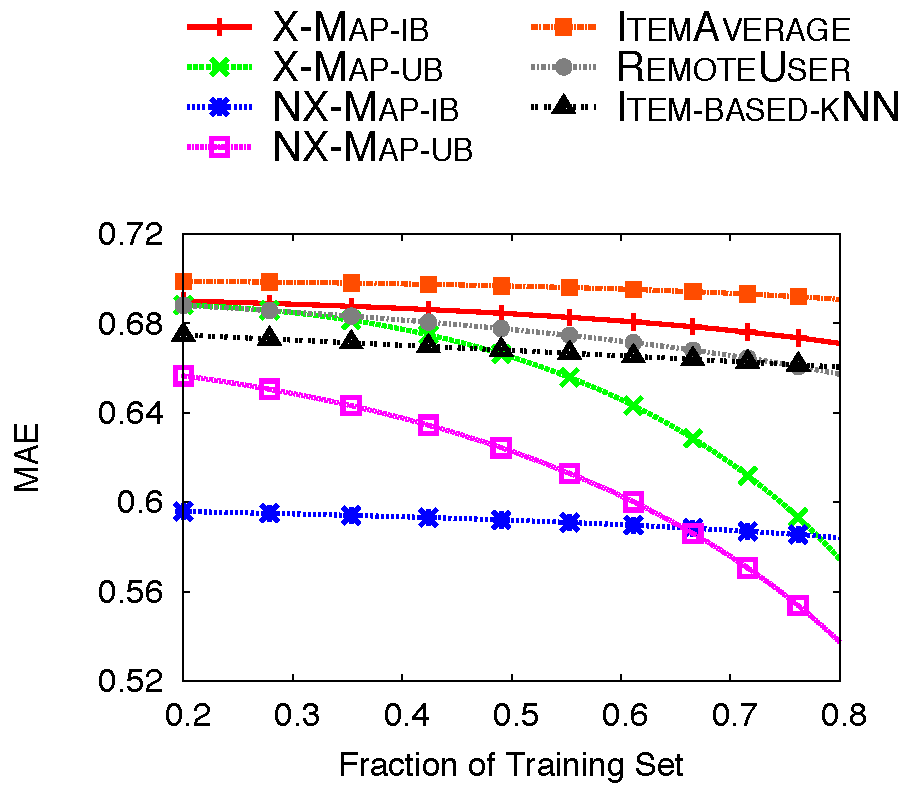
\includegraphics[width=0.245\textwidth,height=0.18\textheight]{figures/MAE_train_original.pdf}}\hspace{-1em}
\subfigure[\it \small Source:Movie, Target:Book \label{fig:Movie2BookvaryTrain}]{\raisebox{1.2mm}{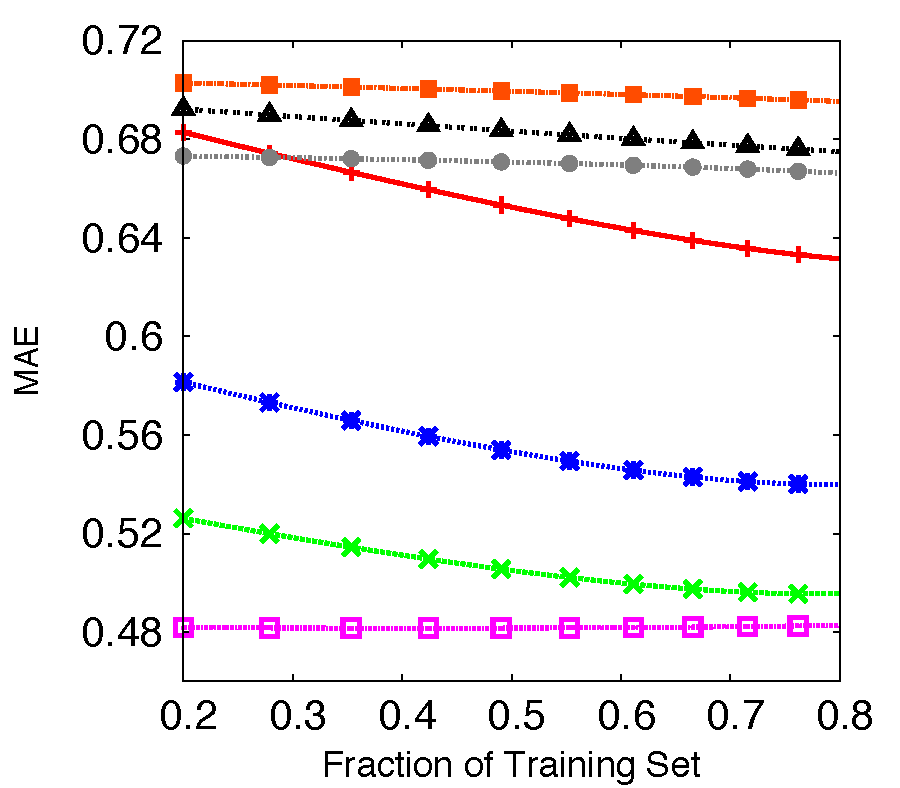
\includegraphics[width=0.245\textwidth,height=0.128\textheight]{figures/MAE_train_swapped.pdf}}}
\vspace{-6mm}
\caption{\bf MAE comparison (Overlap size).\protect\footnotemark}
\label{fig:varyTrain}
\end{figure}

\noindent{\bf Impact of sparsity.}
Next, we evaluate how \crossrec performs when the size of the test profile, in the target domain, increases from a minimum of 0 (cold-start situation) to a maximum of 6 (low sparsity). This experiment also demonstrates the performance of \crossrec when the sparsity of the dataset decreases. Additionally, we evaluate the accuracy improvement of \crossrec over a single domain solution, \emph{item-based kNN in target domain} denoted by \textsc{KNN-sd}, as well over a heterogeneous solution, \emph{item-based kNN in aggregated domain} denoted by \textsc{KNN-cd}. Figure~\ref{fig:varyProfile} demonstrates that \textsc{KNN-sd} and \textsc{KNN-cd} are outperformed by \npcrossrec and \crossrec. Furthermore, we observe a relatively fast improvement for our non-private item-based technique (\npcrossrecib) due to the improvement in item similarities with lower sparsity.
\begin{figure}[ht]
\vspace{-4mm}
\subfigure[\it \small Source:Book, Target:Movie \label{fig:Book2MovievaryProfile}]{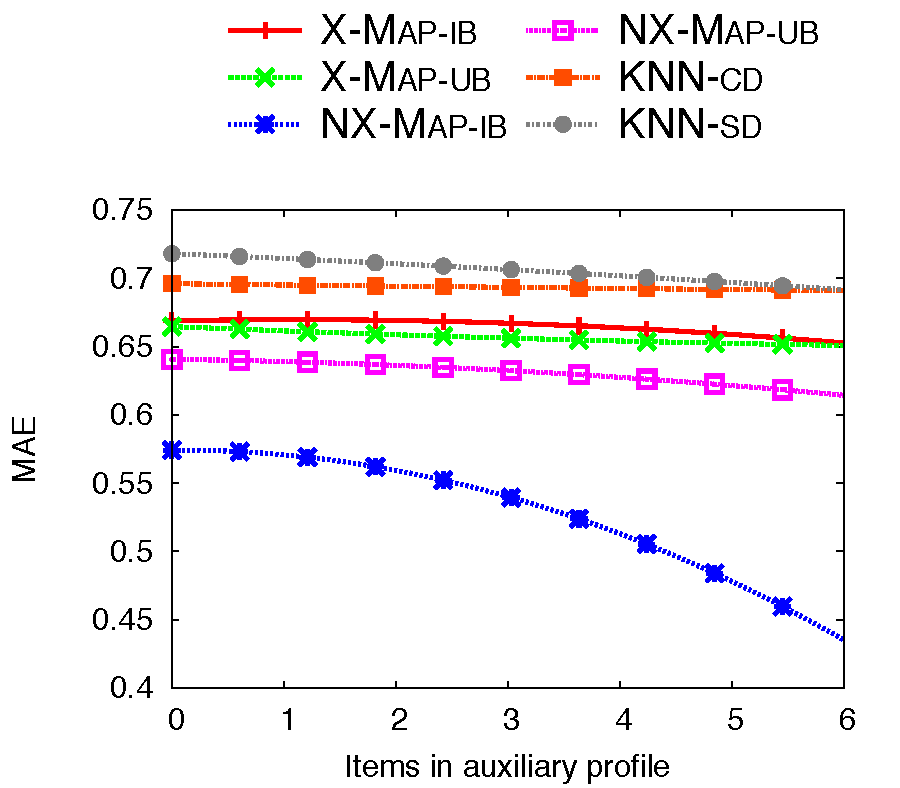
\includegraphics[width=0.245\textwidth,height=0.18\textheight]{figures/MAE_cold_start_original.pdf}}\hspace{-1em}
\subfigure[\it \small Source:Movie, Target:Book \label{fig:Movie2BookvaryProfile}]{\raisebox{1.1mm}{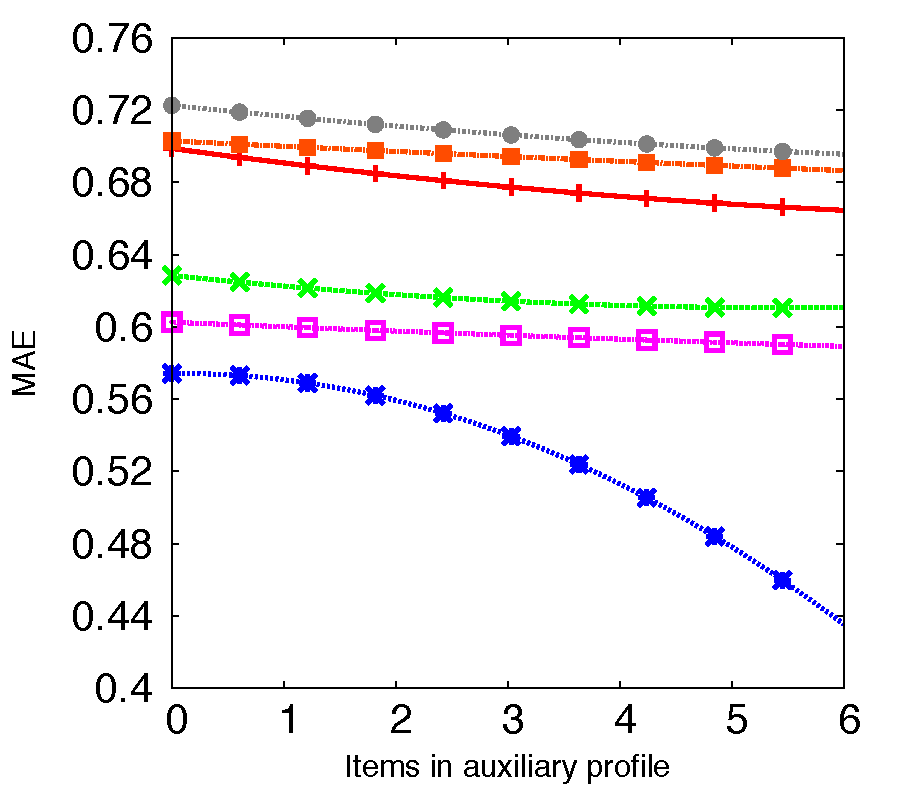
\includegraphics[width=0.245\textwidth,height=0.134\textheight]{figures/MAE_cold_start_swapped.pdf}}}
\vspace{-6mm}
\caption{\bf MAE comparison based on profile size.}
\vspace{2mm}
\label{fig:varyProfile}
\end{figure}

%footnote for overlap size (moved due to page constraint)
\footnotetext{Training set size denotes overlap size.}


\subsection{Scalability}
In this section, we evaluate the scalability of \crossrec in terms of the speedup achieved with an increasing number of computational nodes. We also compare our scalability with a state-of-the-art homogeneous recommender leveraging Spark to implement \emph{Alternating-Least-Squares} based matrix factorization (\textsc{MLlib-ALS}). For the ALS recommender, we use the aggregated ratings over both the domains (Linked-domain personalization). Figure~\ref{fig:scalability} demonstrates the near-linear speedup of \crossrec. Additionally, we see that \crossrec outperforms the scalability achieved by \textsc{MLlib-ALS}.

\begin{figure}[ht]
\vspace{-2mm}
\begin{center}
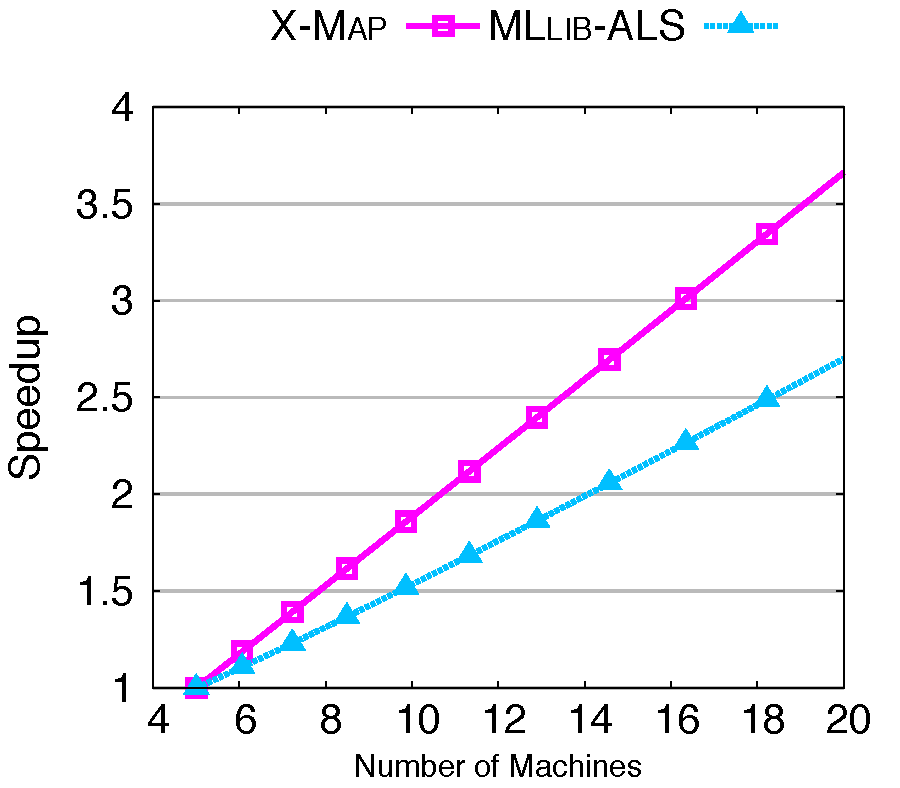
\includegraphics[height=1.3in,width=2in]{figures/Scalability.pdf}
\vspace{-4mm}
\caption{{\bf Scalability of \crossrec.}}
\vspace{-6mm}
\label{fig:scalability}
\end{center}
\end{figure}


\subsection{Online Deployment}
We deployed an online recommendation platform (\url{http://x-map.work/}) leveraging \graphsim and made it available to users. We observe that this recommender is able to recommend books like \emph{Shutter Island: A Novel} when the user queries for the movie \emph{Inception}. Besides, it also recommends the \emph{Shutter Island} movie as a homogeneous recommendation. We observe similar results for multiple other queries. Hence, \graphsim is significantly efficient in achieving heterogeneous personalization in practise.


\iffalse
We deployed a real-time recommender implementing the underlying \graphsim and made it available to internet users. We collected user feedback for a duration of one week which is summarized in Figure~\ref{fig:feedback}. The x-axis denotes the score, provided by the user, in terms of a rating scale ($1$-$5$) with increment of 0.5 and the y-axis denotes the percentage of the total number of users. This preliminary study shows that the user satisfaction level is high.

\begin{figure}[ht]
\vspace{-4mm}
\begin{center}
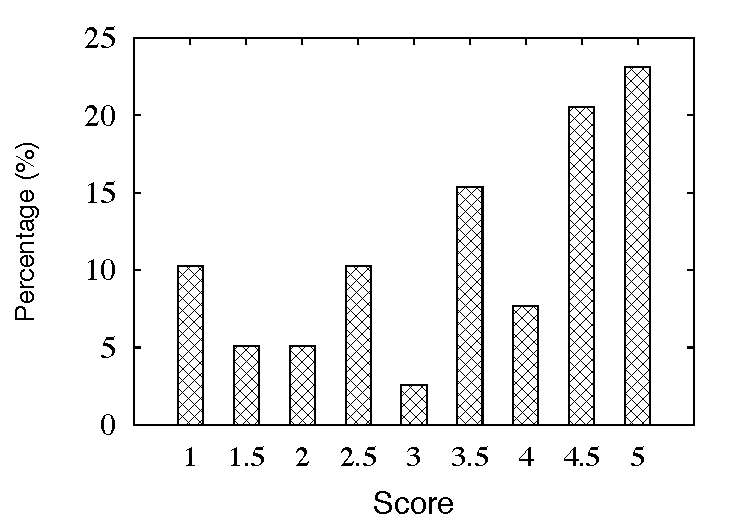
\includegraphics[height=1.3in,width=2in]{figures/Feedback_Frac.pdf}
\vspace{-4mm}
\caption{{\bf Feedback from $51$ users over 1 week.}}
\label{fig:feedback}
\end{center}
\end{figure}
\fi